% INTRODUCTION:
% Thank you very much, my name is Patrick Kraft and I am a PhD Candidate at the Department for Political Science at Stony Brook University. My research is located at the intersection of political behavior and methodology. In my dissertation, I analyze how citizens discuss their political beliefs in their own words. Verbally expressing your attitudes toward an issue is one of the most ubiquitous ways to engage in politics. Yet little research directly studies this basic feature of day-to-day political life. Building on recent advances in quantitative text analysis methods, I develop measures to systematically examine verbatim political attitude expression. A key argument in my thesis is that by analyzing how citizens describe their beliefs and discuss them with peers, we can make inferences about the nature of their attitudes. The research that I want to present today is one chapter out of my dissertations which focuses on political sophistication. I propose a new measure of political sophistication based on verbatim attitude expression in open-ended survey items.

%\begin{frame}{Introduction}
%\begin{itemize}
%\item Verbally \emph{expressing your attitudes} toward an issue is one of the most ubiquitous---yet rarely studied---ways to engage in politics.
%\item<2-> We can leverage how citizens talk about politics to make inferences about the \emph{nature of their attitudes}.
%\vspace{1em}
%\visible<3->{\begin{center}
%\emph{Words} do the work of \emph{politics}\\{\tiny\citep{graham2009liberals}}
%\end{center}}
%\vspace{1em}
%\item<4-> \emph{Research} program:
%\begin{enumerate}
%\item<5-> Study \emph{moralization} in political attitude expression
%\item \only<6-7>{Utilize open-ended responses to measure political \emph{sophistication}}\only<8>{\textbf{Utilize open-ended responses to measure political \emph{sophistication}}}
%\item<7-> Map \emph{social influence} processes in political \emph{discussions}
%\end{enumerate}
%\end{itemize}
%\end{frame}
%
%\begin{frame}{Overview}
%\tableofcontents[hideallsubsections]
%\end{frame}

\begin{frame}{Who scores higher on political knowledge?}
    \begin{center}
        \begin{tikzpicture}
            \node<1>[anchor=south west,inner sep=0] (image) at (0,0) {\includegraphics[width=.9\textwidth]{fig/Respondents0.png}};
            \node<2>[anchor=south west,inner sep=0] (image) at (0,0) {\includegraphics[width=.9\textwidth]{fig/Respondents1.png}};
            \node<3>[anchor=south west,inner sep=0] (image) at (0,0) {\includegraphics[width=.9\textwidth]{fig/Respondents2.png}};
            \node<4>[anchor=south west,inner sep=0] (image) at (0,0) {\includegraphics[width=.9\textwidth]{fig/Respondents3.png}};
            \node<5>[anchor=south west,inner sep=0] (image) at (0,0) {\includegraphics[width=.9\textwidth]{fig/Respondents4.png}};
            \node<6>[anchor=south west,inner sep=0] (image) at (0,0) {\includegraphics[width=.9\textwidth]{fig/Respondents5.png}};
            \node<7>[anchor=south west,inner sep=0] (image) at (0,0) {\includegraphics[width=.9\textwidth]{fig/Respondents6.png}};
            \node<8>[anchor=south west,inner sep=0] (image) at (0,0) {\includegraphics[width=.9\textwidth]{fig/Respondents7.png}};
            \node<9->[anchor=south west,inner sep=0] (image) at (0,0) {\includegraphics[width=.9\textwidth]{fig/Respondents8.png}};
            \node<10->[align=center,draw opacity=0,fill opacity=0.8,text opacity=1, white, fill=beamer@sbred] at (image.center) {\large Both respondents scored \\\Large\textbf{\color{red}{equally}}
            \\\large on the conventional political knowledge measure
            \\\large in the 2012 ANES!};
        \end{tikzpicture}
    \end{center}
\end{frame}

% OLD: I am interested in how individuals describe and justify their political attitudes, which can have important effects, especially in a social context. In my dissertation, I work a lot with open-ended responses.
% OLD: mention data source: ANES 2012, around 5000 respondents, online + f2f study
% I want to start with a little example. I am going to show you two sample responses to open-ended likes/dislikes items in the 2012 American National Election Study. Respondent A and B both described what they liked and disliked about the two major presidential candidates, Barack Obama and Mitt Romney. You know, back in the good old days when Presidential candidates were not considered completely crazy. Respondent A said the following:
% ... Respondent B, on the other hand, said...
% Now, who would you guess scored higher in factual political knowledge? Clearly, our intuition tells us that A seems more knowledgeable than B.

% However, it turns out that these two respondents scored equally on the conventional political knowledge measure in the 2012 ANES!
% factual knowledge: inquiring for example about the number of times an individual can be elected President of the United States, or how the current U.S. federal budget deficit compares to the deficit in the 1990s.

% In this talk, I basically want to convinvce you of two things:
% 1) there is meaningful variance in open-ended responses that is directly related to our conceptualization of political sophistication
% 2) we can gain new insights about the nature of sophistication if we utilize open-ended responses

% So how can we leverage this variation to measure political sophistication in attitude expression:
% Luskin: Sophistication is defined based on a belief system: (1) their \textsl{size} -- i.e. the number of cognitions, (2) their \textsl{range} -- i.e. the dispersion of cognition over categories, and (3) their \textsl{constraint} -- i.e. the extent to which cognitions are interconnected in a meaningful way.``

% How can we measure sophistication based on these open-ended responses? Well, the first possibility would be to read them and code them manually. And while I can tell you that that is quite entertaining for a little while, it is of course very labor intensive, especially in large-scale surveys.

% While I do not want to spend too much time on the methodological details, I basically incorporate three characteristics of open-ended responses that I argue to be related to our understanding of political sophistication:
% 1) relative length
% 2) topic diversity: do respondents only focus on one topic, or do they reference multiple considerations
% 3) opinion diversity: the extent to which individuals are able to discuss positive and negative aspects regarding each candidate

\subsection{Knowledge, Sophistication, and Competence}

\begin{frame}{Conventional Measures of Political Knowledge}
\emph{Definition:} ``The range of factual information about politics that is stored in long-term memory.'' {\footnotesize\cite[10]{carpini1996americans}}
\\\vspace{1em}
\visible<2->{\emph{General finding:} Lack of information among the public
%\begin{itemize}\footnotesize
%\item \cite{converse1964nature}, \cite{carpini1996americans}, \cite{althaus1998information}
%\end{itemize}
}
\\\vspace{2em}
\visible<3->{\emph{Caveat 1:} Measurement issues
%\begin{itemize}\footnotesize
%\item \cite{mondak2001asked}, \cite{pietryka2013analysis}, \cite{barabas2014question}
%\end{itemize}
}
\\\vspace{1em}
\visible<4->{\emph{Caveat 2:} Theoretical relevance
%\begin{itemize}\footnotesize
%\item \cite{luskin1987measuring}, \cite{druckman2014pathologies}, \cite{lupia2015uninformed}
%\end{itemize}
}
% COMMENT: mention the main point first
% Caveat 1: We don't measure it correctly due to personality, differential item functioning, different types of knowledge
% Caveat 2: Factual knowledge is not necessarily theoretically relevant...
\end{frame}
% Druckman: motivation to be accurate as a good standard to evaluate political competence, that implies considering multiple perspectives
% Lupia: knowledge that is asked for is not really necessay
% Delli Carpini and Keeter (1996): more than 5000 citations

\begin{frame}{Discursive Sophistication and Competence}
Verbatim political \emph{attitude expression}:
\begin{itemize}[<+->]
\item \emph{Communication} and information diffusion
\item Reflects \emph{political belief system} \& \emph{accuracy motivation}
\item Capture \emph{salient} issues, available \emph{frames}, and related \emph{considerations}
\item Measure sophistication related to specific \emph{political tasks}
%\\\emph{\faArrowRight\hspace{.1em}}Structure of \emph{political belief systems}
\item Fewer \emph{assumptions} about necessary pieces of information
\end{itemize}\vspace{2em}
\onslide<6->{\emph{\faArrowRight\hspace{.1em}} A \emph{Naive} Approach for Measuring \emph{Sophistication}}
\end{frame}
% We can look at how they \emph{discuss} their political \emph{preferences} in their \emph{own words}
% Rather than looking at factual knowledge that always involves assumptions about what people should know and how they should react to certain information
% Most studies that are interested in political sophistication focus on conventional factual knowledge scores as proxies. However, these measures have been criticized from theoretical and measurement perspectives. Lupia, for example, argues that the factual information asked for often has now apparent relevance to perform political tasks. The approach that I propose is naive in that it does not presuppose a set of information that is deemed necessary. Rather, it tries to quantify the complexity of individual attitude expressions related to a political task.



\subsection{Measuring Discursive Sophistication}

\begin{frame}
    \begin{center}
        \begin{tikzpicture}
            \node[anchor=south west,inner sep=0] (image) at (0,0) {\includegraphics[width=.9\textwidth]{fig/Respondents_empty.png}};
            \node[align=center] at (image.center) {\Large \emph{Measuring Discursive Sophistication}};
        \end{tikzpicture}
    \end{center}
\end{frame}

% INTRODUCTION
% Work on transition for discursive sophistication

\begin{frame}{Discursive Sophistication
	\only<1-3>{-- Components}\only<4-5>{-- Structural Topic Model}\label{overview_stm}\only<6->{-- Components}}
\begin{center}
        \begin{tikzpicture}
            \node<1-4>[anchor=south west,inner sep=0] (image) at (0,0) {\includegraphics[width=\textwidth]{fig/lda_empty.pdf}};
            \node<2-3>[align=left] (image) at (9,4) {
            	\only<2->{\emph{\faCaretRight} \hyperlink{opinionation}{\emph{Opinionation}}\\
            	Does a respondent discuss all questions?}\\\\
            	\only<3->{\emph{\faCaretRight} \hyperlink{elaboration}{\emph{Considerations}}\\
            	How many topics are mentioned?}\\\\
            	\only<5->{\emph{\faCaretRight} \hyperlink{eloquence}{\emph{Word Choice}}\\
            	Are terms highly descriptive of topics?}
        		};
            \node<4>[align=left] (image) at (9,4) {
            \emph{Processing} open-ended responses:\\
            \emph{\faCaretRight} Automatic spell checking\\
            \emph{\faCaretRight} Lower case\\
            \emph{\faCaretRight} Stopwords, Numbers, Punctuation\\
            \emph{\faCaretRight} Stemming\\
            \emph{\faCaretRight} Infrequent terms\\
            \emph{\faCaretRight} Aggregation \vspace{1em}\\
            \emph{\faArrowRight} \emph{Structural topic model}\\ {\footnotesize\citep{roberts2014structural}}};
            \node<5>[anchor=south west,inner sep=0] (image) at (0,0) {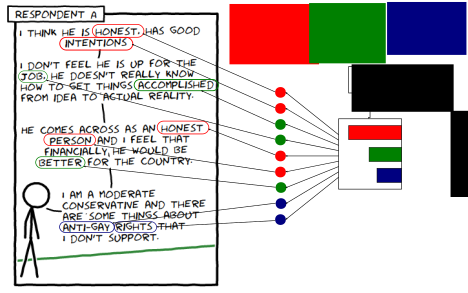
\includegraphics[width=\textwidth]{fig/lda.pdf}};
            \node<6->[anchor=south west,inner sep=0] (image) at (0,0) {\includegraphics[width=\textwidth]{fig/lda_empty.pdf}};
            \node<6->[align=left] (image) at (9,4) {
            	\only<6->{\emph{\faCaretRight} \hyperlink{opinionation}{\emph{Opinionation}}\\
            		Does a respondent discuss all questions?}\\\\
            	\only<6->{\emph{\faCaretRight} \hyperlink{elaboration}{\emph{Considerations:}}\\
            		How many topics are mentioned?}\\\\
            	\only<6->{\emph{\faCaretRight} \hyperlink{eloquence}{\emph{Word Choice:}}\\
            		Are terms highly descriptive of topics?}
            };
        \end{tikzpicture}
    \end{center}
%\visible<2>{\flushright\small \cite{roberts2014structural}}
%\flushright{\footnotesize\texttt{\textcolor{gray}{\hyperlink{components}{[back]}}}}
\end{frame}

%\begin{frame}{Discursive Sophistication -- Components}\label{components}
%\visible<1->{Extracted \emph{Quantities}:
%\begin{enumerate}
%\item \hyperlink{opinionation}{\emph{Opinionation:}} Does a respondent discuss all questions?
%\item<2-> \hyperlink{elaboration}{\emph{Considerations:}} How many topics are mentioned?
%\item<4-> \hyperlink{eloquence}{\emph{Word Choice:}} Are terms highly descriptive of topics? 
%
%\end{enumerate}}
%
%\only<3>{
%\begin{textblock*}{54mm}(7mm,0.65\textheight)
%\begin{exampleblock}{Few Considerations}
%    {\color{green!50!black}{Represents all people.}}
%    \\{\color{red}{Represent the rich.}}
%    \\{\color{green!50!black}{Represents the working class.}}
%    \\{\color{red}{Represents the wealthy.}}
%\end{exampleblock}
%\end{textblock*}
%\begin{textblock*}{54mm}(67mm,0.65\textheight)
%\begin{exampleblock}{Many Considerations}
%	{\color{green!50!black}{Everything.}}
%	\\{\color{red}{Attitude toward women's rights, view on taxes mainly.}}
%	\\{\color{green!50!black}{Has more people that I trust.}}
%	\\{\color{red}{Too conservative.}}
%\end{exampleblock}
%\end{textblock*}
%} % Answers between 10 and 20 terms, min vs. max elaboration
%
%\only<5>{
%\begin{textblock*}{54mm}(7mm,0.65\textheight)
%\begin{exampleblock}{Low Descriptiveness}
%  enthus\\standoffish\\endless
%\end{exampleblock}
%\end{textblock*}
%\begin{textblock*}{54mm}(67mm,0.65\textheight)
%\begin{exampleblock}{High Descriptiveness}
%  health\\tax\\economi
%\end{exampleblock}
%\end{textblock*}
%} % Individual terms ranked highest and lowest on distinctiveness
%
%\end{frame}
%% add examples for each dimension here


%\subsection{Relationship Between Individual Sophistication Components}
\begin{frame}{\hyperlink{corplot}{Discursive Sophistication -- Components (2012 ANES)}}\label{corplot_components}
\begin{center}
        \begin{tikzpicture}
            \node<1>[anchor=south west,inner sep=0] (image) at (0,0) {\includegraphics[height=.85\textheight]{../fig/anes2012_corplot_components0.pdf}};
            \node<2->[anchor=south west,inner sep=0] (image) at (0,0) {\includegraphics[height=.85\textheight]{../fig/anes2012_corplot_components.pdf}};
            \node<3>[align=center,draw opacity=0,fill opacity=0.8,text opacity=1, white, fill=beamer@sbred] at (image.center) {Discursive Sophistication\\=\\ $\tfrac{1}{3}$(Opinionation + Considerations + Word Choice)};
        \end{tikzpicture}
    \end{center}
%\visible<2>{\flushright\small \cite{roberts2014structural}}
%\flushright{\footnotesize\texttt{\textcolor{gray}{\hyperlink{components}{[back]}}}}
\end{frame}


